\section{moSteadyFitSolContinue$<$ EOT $>$ Class Template Reference}
\label{classmo_steady_fit_sol_continue}\index{moSteadyFitSolContinue@{moSteadyFitSolContinue}}
One possible stopping criterion for a solution-based heuristic.  


{\tt \#include $<$moSteadyFitSolContinue.h$>$}

Inheritance diagram for moSteadyFitSolContinue$<$ EOT $>$::\begin{figure}[H]
\begin{center}
\leavevmode
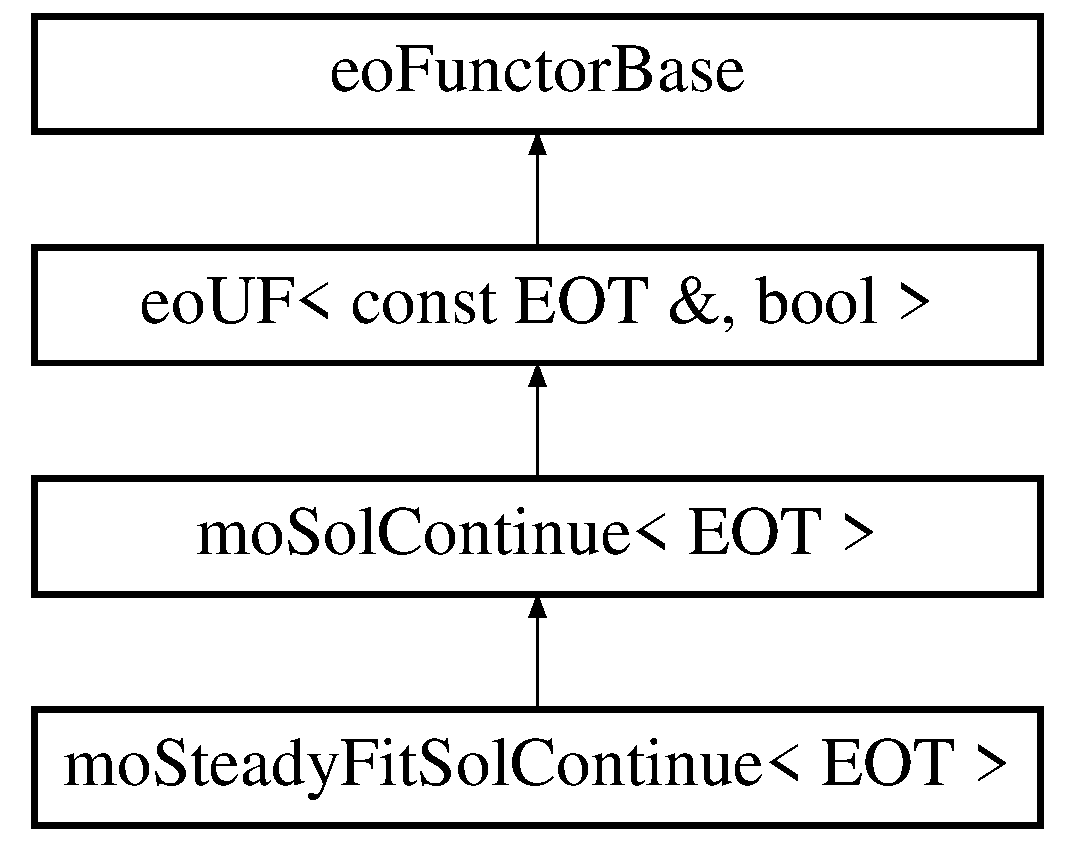
\includegraphics[height=4cm]{classmo_steady_fit_sol_continue}
\end{center}
\end{figure}
\subsection*{Public Types}
\begin{CompactItemize}
\item 
typedef EOT::Fitness {\bf Fitness}\label{classmo_steady_fit_sol_continue_c289721abbbafe50f6e3b8305dd31007}

\begin{CompactList}\small\item\em Alias for the fitness. \item\end{CompactList}\end{CompactItemize}
\subsection*{Public Member Functions}
\begin{CompactItemize}
\item 
{\bf moSteadyFitSolContinue} (unsigned int \_\-\_\-maxNumberOfIterations, unsigned int \_\-\_\-maxNumberOfIterationWithoutImprovement, bool \_\-\_\-minimization=true)
\begin{CompactList}\small\item\em Basic constructor. \item\end{CompactList}\item 
bool {\bf operator()} (const EOT \&\_\-\_\-sol)
\begin{CompactList}\small\item\em Function that activates the stopping criterion. \item\end{CompactList}\item 
void {\bf init} ()\label{classmo_steady_fit_sol_continue_87563493addc8e4b58982c55a67179b9}

\begin{CompactList}\small\item\em Procedure which allows to initialise the stuff needed. \item\end{CompactList}\end{CompactItemize}
\subsection*{Private Attributes}
\begin{CompactItemize}
\item 
unsigned int {\bf maxNumberOfIterations}\label{classmo_steady_fit_sol_continue_36b43c2a252887ad027165ac32393fe8}

\begin{CompactList}\small\item\em Maximum number of iterations before considering the fitness. \item\end{CompactList}\item 
unsigned int {\bf maxNumberOfIterationsWithoutImprovement}\label{classmo_steady_fit_sol_continue_cde593c09f497a5fa66ff62732544f40}

\begin{CompactList}\small\item\em Maximum number of iterations without improvement allowed. \item\end{CompactList}\item 
bool {\bf maxNumberOfIterationsReached}\label{classmo_steady_fit_sol_continue_7d88c0eb91b2a12121ba1c3ae9139887}

\begin{CompactList}\small\item\em Flag that indicates that the maxNumberIteration have been reached. \item\end{CompactList}\item 
bool {\bf firstFitnessSaved}\label{classmo_steady_fit_sol_continue_025bf2789e470fdde989eee9121035c3}

\begin{CompactList}\small\item\em Flag that this is the first time that the fitness is used. \item\end{CompactList}\item 
{\bf Fitness} {\bf fitness}\label{classmo_steady_fit_sol_continue_a5c62e7049b36f6e71e92b559568c09e}

\begin{CompactList}\small\item\em Current Fitness. \item\end{CompactList}\item 
bool {\bf minimization}
\begin{CompactList}\small\item\em Flag that indicate if there is a minimization (true) or a maximization (false) of the fitness value. \item\end{CompactList}\item 
unsigned int {\bf counter}\label{classmo_steady_fit_sol_continue_245c9099a2c40dfc4f34b3ff216d13ce}

\begin{CompactList}\small\item\em The iteration couter. \item\end{CompactList}\end{CompactItemize}


\subsection{Detailed Description}
\subsubsection*{template$<$class EOT$>$ class moSteadyFitSolContinue$<$ EOT $>$}

One possible stopping criterion for a solution-based heuristic. 

The stop criterion corresponds to a maximum number of iterations without improvement (after a minimum number of iterations). 



Definition at line 21 of file moSteadyFitSolContinue.h.

\subsection{Constructor \& Destructor Documentation}
\index{moSteadyFitSolContinue@{moSteadyFitSolContinue}!moSteadyFitSolContinue@{moSteadyFitSolContinue}}
\index{moSteadyFitSolContinue@{moSteadyFitSolContinue}!moSteadyFitSolContinue@{moSteadyFitSolContinue}}
\subsubsection{\setlength{\rightskip}{0pt plus 5cm}template$<$class EOT$>$ {\bf moSteadyFitSolContinue}$<$ EOT $>$::{\bf moSteadyFitSolContinue} (unsigned int {\em \_\-\_\-maxNumberOfIterations}, unsigned int {\em \_\-\_\-maxNumberOfIterationWithoutImprovement}, bool {\em \_\-\_\-minimization} = {\tt true})\hspace{0.3cm}{\tt  [inline]}}\label{classmo_steady_fit_sol_continue_0c7e09ca080bfb1dd493015d23a50ad7}


Basic constructor. 

\begin{Desc}
\item[Parameters:]
\begin{description}
\item[{\em \_\-\_\-maxNumberOfIterations}]The number of iterations to reach before looking for the fitness. \item[{\em \_\-\_\-maxNumberOfIterationWithoutImprovement}]The number of iterations without fitness improvement to reach for stop. \item[{\em \_\-\_\-minimization}]Indicate if the the aim is to maximize or minimize the fitness. \end{description}
\end{Desc}


Definition at line 35 of file moSteadyFitSolContinue.h.

\subsection{Member Function Documentation}
\index{moSteadyFitSolContinue@{moSteadyFitSolContinue}!operator()@{operator()}}
\index{operator()@{operator()}!moSteadyFitSolContinue@{moSteadyFitSolContinue}}
\subsubsection{\setlength{\rightskip}{0pt plus 5cm}template$<$class EOT$>$ bool {\bf moSteadyFitSolContinue}$<$ EOT $>$::operator() (const EOT \& {\em \_\-\_\-sol})\hspace{0.3cm}{\tt  [inline, virtual]}}\label{classmo_steady_fit_sol_continue_942e58ec00bb61000a83c80176e14bc3}


Function that activates the stopping criterion. 

Indicates if the fitness has not been improved since a number of iterations (after a minimum of iterations).

\begin{Desc}
\item[Parameters:]
\begin{description}
\item[{\em \_\-\_\-sol}]the current solution. \end{description}
\end{Desc}
\begin{Desc}
\item[Returns:]true or false. \end{Desc}


Implements {\bf eoUF$<$ const EOT \&, bool $>$}.

Definition at line 47 of file moSteadyFitSolContinue.h.

References moSteadyFitSolContinue$<$ EOT $>$::counter, moSteadyFitSolContinue$<$ EOT $>$::firstFitnessSaved, moSteadyFitSolContinue$<$ EOT $>$::fitness, moSteadyFitSolContinue$<$ EOT $>$::maxNumberOfIterations, moSteadyFitSolContinue$<$ EOT $>$::maxNumberOfIterationsReached, moSteadyFitSolContinue$<$ EOT $>$::maxNumberOfIterationsWithoutImprovement, and moSteadyFitSolContinue$<$ EOT $>$::minimization.

\subsection{Member Data Documentation}
\index{moSteadyFitSolContinue@{moSteadyFitSolContinue}!minimization@{minimization}}
\index{minimization@{minimization}!moSteadyFitSolContinue@{moSteadyFitSolContinue}}
\subsubsection{\setlength{\rightskip}{0pt plus 5cm}template$<$class EOT$>$ bool {\bf moSteadyFitSolContinue}$<$ EOT $>$::{\bf minimization}\hspace{0.3cm}{\tt  [private]}}\label{classmo_steady_fit_sol_continue_4176d8cc6fda6cb854997a845faaf8a4}


Flag that indicate if there is a minimization (true) or a maximization (false) of the fitness value. 

It can be interesting to know this information because some solution-based metaheuristics can generate solution with a fitness that is worse that the best known fitness (in this case, the counter is not reinitialized). 

Definition at line 114 of file moSteadyFitSolContinue.h.

Referenced by moSteadyFitSolContinue$<$ EOT $>$::operator()().

The documentation for this class was generated from the following file:\begin{CompactItemize}
\item 
moSteadyFitSolContinue.h\end{CompactItemize}
